\section*{Übung 5}
\subsection*{Aufgabe 1}
\subsubsection*{Lösungsidee}
Beim Telefonverzeichnis werden Procedures geschrieben die das Verwalten eines Telefonverzeichnisses vereinfachen. Dabei wird ein Typ Entry und ein Array verwendet. Mithilfe der Procedures wird auf das dictionary zugegriffen und verändert.
\newline

\lstinputlisting[language=Pascal] {../phonedictionary.pas}
\begin{figure}[H]
	\centering
	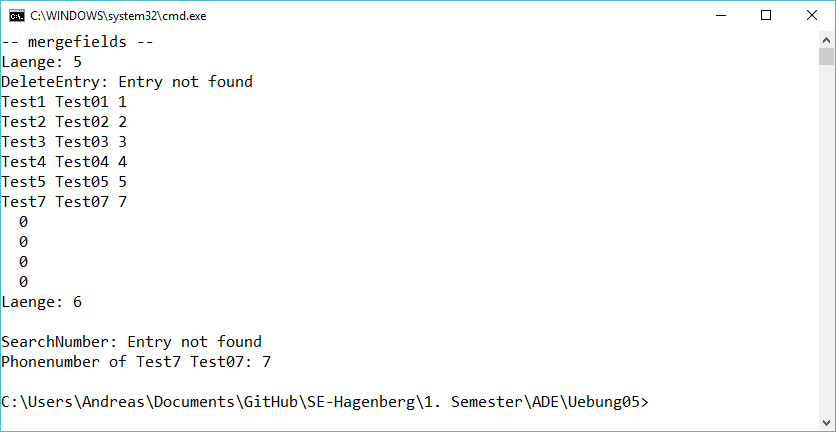
\includegraphics[scale=0.75]{./pictures/phonedictionary.png}
	\caption{Testfälle Phonedictionary}
	\label{fig: phonedictionary}
\end{figure}

\section*{Testfälle}
Es werden alle Funktionen und Procedures getestet, auch auf falsche Eingaben.

\newpage

\subsection*{Aufgabe 2}
\subsubsection*{Lösungsidee}
Zuerst wird das erste Array durchsucht und alle Zahlen die nicht in dem zweiten Array vorkommen werden in das dritte Array geschrieben. Dadurch das die beiden ersten Arrays sortiert sind ist das dritte Array nah dem einfügen auch sortiert. Danach wird beim Durchlauf des zweiten Arrays alle Zahlen die nicht im ersten Array vorkommen geordnet in das dritte Array eingefügt.
\newline

\lstinputlisting[language=Pascal] {../mergefields.pas}
\begin{figure}[H]
	\centering
	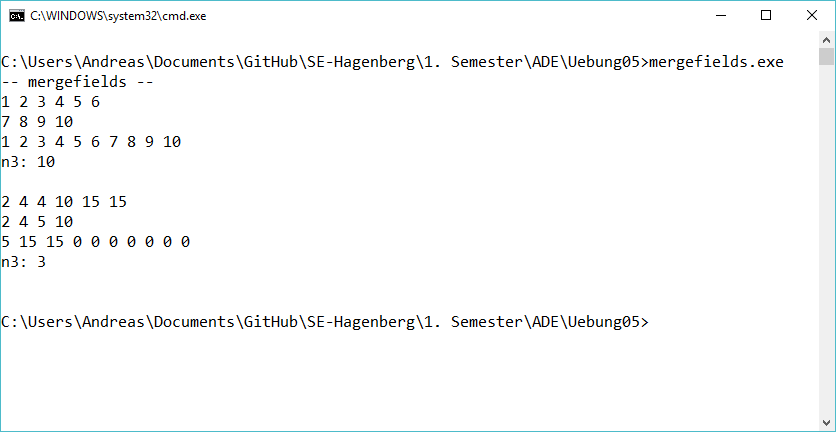
\includegraphics[scale=0.75]{./pictures/mergefields.png}
	\caption{Testfälle Mergefeilds}
	\label{fig: mergefields}
\end{figure}

\section*{Testfälle}
Zwei verschiedene Arrays, mit unterschiedlichen Zahlen bei denen Mergesort durchgeführt wird.

\newpage
